\chapter{Grundlagen}
\label{Kap2}

\section{Progressive Web App}
Eine \ac{PWA} ist eine Anwendung, die in modernen Webbrowsern läuft und dem Nutzer dabei eine Erfahrung ähnlich zu bekannten nativen Apps bietet \autocite{Sheppard2017} \autocite{Rojas2020}. Die wichtigsten Funktionen dabei sind:

\begin{itemize}
  \item Schnell: Die App startet schnell und bietet schnell die Möglichkeit zur Interkation \autocite{Hajian2019} \autocite{Sheppard2017}
  \item Zuverlässig: auf älteren Geräten funktionsfähig und auch ohne Internet nutzbar. Außerdem passt sich das Design an verschiedene Bildschirmgrößen an (responsive design) \autocite{Hajian2019} \autocite{Sheppard2017}
  \item Installierbar: nach dem Installieren wird ein Icon auf dem Homescreen angezeigt \autocite{Hajian2019} \autocite{Sheppard2017} \autocite{Rojas2020}
  \item Benachrichtigungen: der Nutzer kann Benachrichtigungen bekommen, obwohl er die App nicht offen hat und aktiv benutzt \autocite{Hajian2019} \autocite{Sheppard2017} 
  \item Native-like Funktionen: Zugriff auf Hardware wie zum Beispiel die Kamera \autocite{Hajian2019}
\end{itemize}

Bei der Nutzung bzw. der Entwicklung einer \ac{PWA} entstehen viele Vorteile für die Entwickler und Nutzer. Webtechnologien sind weit verbreitet und für jedes Betriebssystem sind moderne Browser verfügbar, dadurch kann die Anwendung sehr leicht an eine große Nutzergruppe ausgeliefert werden \autocite{Rojas2020}. Das Ausliefern an die Nutzer ist auch sehr einfach, weil diese nur eine URL benötigen \autocite{KHAN2019289} und eine neue Version der App automatisch beim Start der App heruntergeladen wird \autocite{Rojas2020}. Außerdem ist die Entwicklung mit Webtechnologien weit verbreitet, man findet viele Ressourcen und Tools, die bei der Entwicklung helfen \autocite{Rojas2020}. Beim Vergleichen von nativen Apps zu einer \ac{PWA} fällt zudem auf, dass die \ac{PWA} sehr wenig Speicherplatz nach der Installation benötigt \autocite{biorn2017} \autocite{KHAN2019289}. Die Geschwindigkeit einer \ac{PWA} auf Android kann im Vergleich zu anderen Cross-Platform Ansätzen mithalten oder ist sogar schneller \autocite{biorn2017}.

Eine \ac{PWA} hat nicht nur Vorteile, sondern auch Nachteile. Einer davon ist die Limitierung auf die APIs der Webbrowser. Hinzu kommt, dass einige Funktionen noch nicht standardisiert sind und / oder noch nicht von allen gängigen Browsern unterstützt werden \autocite{majchrzak2018} \autocite{biorn2017}. Wenn die Performance der App eine große Rolle spielt, wie etwas bei Spielen, ist eine \ac{PWA} nicht sehr gut geeignet \autocite{biorn2017}.

Damit aus einer Website eine \ac{PWA} wird sind mindestens zwei Dinge erforderlich. Erstens wird eine Manifest Datei benötigt, die Informationen über das Icon, den Namen und vielen mehr enthält \autocite{Hajian2019} \autocite{Rojas2020}. Als zweites wird ein Service Worker benötigt, der unter anderem für die Offline-Fähigkeit verantwortlich ist \autocite{Rojas2020}. 


\section{Angular und Typescript}
Angular ist ein Framework zum Entwickeln von Webanwendungen für alle Platformen \autocite{angular-io}. Es ist Open-Source, getrieben von einer großen Community aber auch von Firmen wie Google weiterentwickelt und selbst viel genutzt \autocite{angular-io}. Als Programmiersprache ist Typescript vorgesehen. 

Typescript erweitert JavaScript um einige Funktionen wie zum Beispiel Typisierung \autocite{typescript-org}. Typescript kann vor dem Ausliefern in reines JavaScript kompiliert werden und ist somit in allen gängigen Browsern oder auch auf Servern mit Node.js ausführbar \autocite{typescript-org}.

Die Kombination aus Angular und Typescript bietet eine sehr gute Basis zum Entwickeln von großen, schnellen und skalierbaren Anwendungen \autocite{angular-io}. Durch die statische Typisierung sind zum Beispiel Refactorings mit den vielen verfügbaren Tools schnell und sicher durchzuführen \autocite{typescript-org} \autocite{angular-io}. In der großen Community findet man auf sehr viele Fragen sofort eine Antwort.

\section{CROSSLOAD}
CROSSLOAD ist ein Webportal das christliche Medien, im Moment hauptsächlich Predigten, zur Verfügung stellt \autocite{crossload-org}. Diese Medien können durchsucht, angehört und heruntergeladen werden. Die Entwicklung befindet sich im Moment in der Beta-Phase (https://beta.crossload.org) und wird vor allem von Ehrenamtlichen vorangetrieben. In Abbildung~\ref{Kap3:crossload-mobil-neuste-inhalte} ist die mobile Seite mit den neusten Inhalten auf CROSSLOAD zu sehen. Abbildung~\ref{Kap3:crossload-mobil-detail} zeigt die Detailansicht einer Predigt.

\begin{figure}[ht]
  \centering
  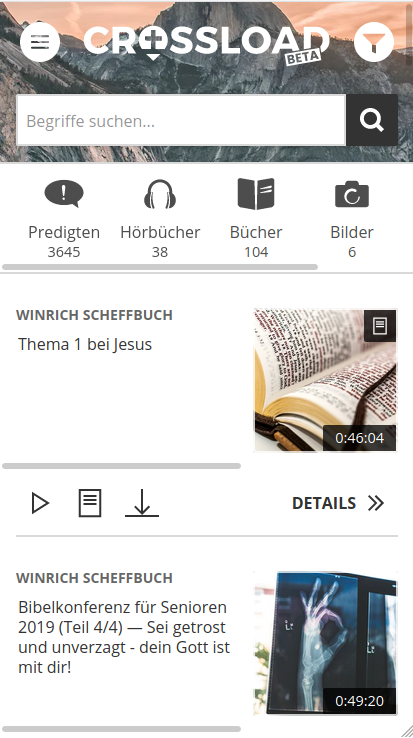
\includegraphics[width=5cm]{crossload-mobil-neuste-inhalte}
  \caption{CROSSLOAD - Mobile Ansicht der neusten Inhalte}
  \label{Kap3:crossload-mobil-neuste-inhalte}
\end{figure}

\begin{figure}[ht]
  \centering
  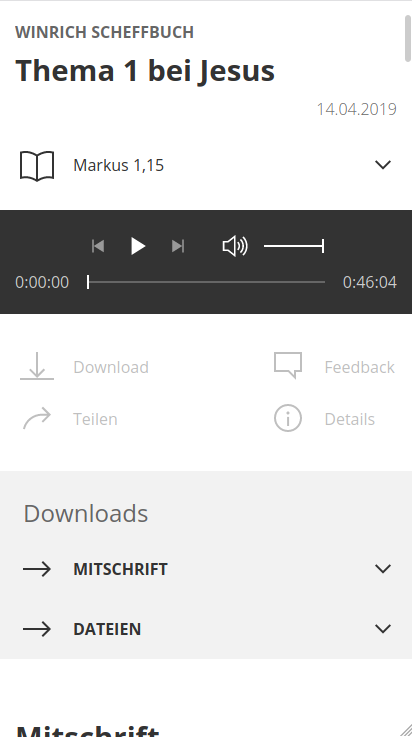
\includegraphics[width=5cm]{crossload-detailansicht}
  \caption{CROSSLOAD - Dateilansicht einer Predigt}
  \label{Kap3:crossload-mobil-detail}
\end{figure}

Im Frontend wird Angular mit Typescript zum Entwickeln verwendet und das Backend besteht aus vielen verschiedenen Services, die mit unterschiedlichen Sprachen und Frameworks entwickelt werden. Für diese Arbeit ist nur die Technologie für das Frontend interessant. Das Webportal besitzt schon über eine Manifest-Datei und kann somit auf den Startbildschirm des Smartphones hinzugefügt werden. Statische Inhalte werden bereits gecached und sind somit auch offline Verfügbar. 
